\documentclass[border=3mm]{standalone}
\usepackage{tikz}
\usetikzlibrary{automata, positioning}
\begin{document}
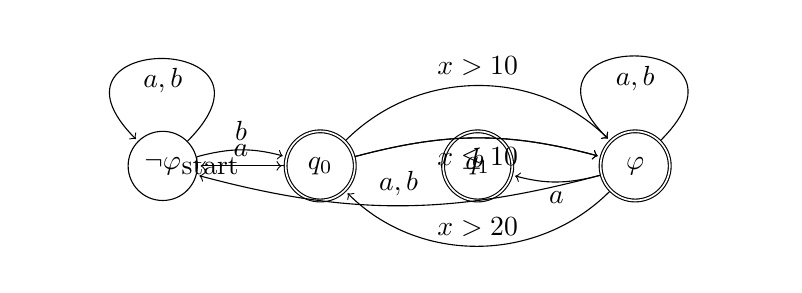
\begin{tikzpicture}[shorten >=1pt,node distance=2cm,on grid,auto]
    \node[state,initial,accepting]   (q0)   {$q_0$};
    \node[state,accepting]           (q1) [right=of q0] {$q_1$};
    \node[state]                     (qa) [left=of q0]  {$\neg \varphi$};
    \node[state,accepting]           (qb) [right=of q1] {$\varphi$};
    \path[->]
        (qa) edge [loop,below] node {$a,b$} ()
             edge[bend left=15] node [above] {$b$} (q0)
        (q0) edge                node [above] {$a$} (qa)
             edge[bend left=15] node [below] {$b$} (qb)
             edge[bend left=45] node [above,sloped] {$x>10$} (qb)
        (qb) edge[bend left=45] node [above,sloped] {$x>20$} (q0)
             edge[bend left=15] node [below] {$a$} (q1)
             edge[loop,below] node {$a,b$} ();
    \path[->]
        (q0) edge[bend left=15] node [below] {$x\leq10$} (qb);
    \path[->]
        (qb) edge[bend left=15] node [above] {$a,b$} (qa);
\end{tikzpicture}
\end{document}